 
%% bare_jrnl.tex
%% V1.4
%% 2012/12/27
%% by Michael Shell
%% see http://www.michaelshell.org/
%% for current contact information.
%%
%% This is a skeleton file demonstrating the use of IEEEtran.cls
%% (requires IEEEtran.cls version 1.8 or later) with an IEEE journal paper.
%%
%% Support sites:
%% http://www.michaelshell.org/tex/ieeetran/
%% http://www.ctan.org/tex-archive/macros/latex/contrib/IEEEtran/
%% and
%% http://www.ieee.org/



% *** Authors should verify (and, if needed, correct) their LaTeX system  ***
% *** with the testflow diagnostic prior to trusting their LaTeX platform ***
% *** with production work. IEEE's font choices can trigger bugs that do  ***
% *** not appear when using other class files.                            ***
% The testflow support page is at:
% http://www.michaelshell.org/tex/testflow/


%%*************************************************************************
%% Legal Notice:
%% This code is offered as-is without any warranty either expressed or
%% implied; without even the implied warranty of MERCHANTABILITY or
%% FITNESS FOR A PARTICULAR PURPOSE!
%% User assumes all risk.
%% In no event shall IEEE or any contributor to this code be liable for
%% any damages or losses, including, but not limited to, incidental,
%% consequential, or any other damages, resulting from the use or misuse
%% of any information contained here.
%%
%% All comments are the opinions of their respective authors and are not
%% necessarily endorsed by the IEEE.
%%
%% This work is distributed under the LaTeX Project Public License (LPPL)
%% ( http://www.latex-project.org/ ) version 1.3, and may be freely used,
%% distributed and modified. A copy of the LPPL, version 1.3, is included
%% in the base LaTeX documentation of all distributions of LaTeX released
%% 2003/12/01 or later.
%% Retain all contribution notices and credits.
%% ** Modified files should be clearly indicated as such, including  **
%% ** renaming them and changing author support contact information. **
%%
%% File list of work: IEEEtran.cls, IEEEtran_HOWTO.pdf, bare_adv.tex,
%%                    bare_conf.tex, bare_jrnl.tex, bare_jrnl_compsoc.tex,
%%                    bare_jrnl_transmag.tex
%%*************************************************************************

% Note that the a4paper option is mainly intended so that authors in
% countries using A4 can easily print to A4 and see how their papers will
% look in print - the typesetting of the document will not typically be
% affected with changes in paper size (but the bottom and side margins will).
% Use the testflow package mentioned above to verify correct handling of
% both paper sizes by the user's LaTeX system.
%
% Also note that the "draftcls" or "draftclsnofoot", not "draft", option
% should be used if it is desired that the figures are to be displayed in
% draft mode.
%
\documentclass[journal]{IEEEtran}
%
% If IEEEtran.cls has not been installed into the LaTeX system files,
% manually specify the path to it like:
% \documentclass[journal]{../sty/IEEEtran}





% Some very useful LaTeX packages include:
% (uncomment the ones you want to load)


% *** MISC UTILITY PACKAGES ***
%
%\usepackage{ifpdf}
% Heiko Oberdiek's ifpdf.sty is very useful if you need conditional
% compilation based on whether the output is pdf or dvi.
% usage:
% \ifpdf
%   % pdf code
% \else
%   % dvi code
% \fi
% The latest version of ifpdf.sty can be obtained from:
% http://www.ctan.org/tex-archive/macros/latex/contrib/oberdiek/
% Also, note that IEEEtran.cls V1.7 and later provides a builtin
% \ifCLASSINFOpdf conditional that works the same way.
% When switching from latex to pdflatex and vice-versa, the compiler may
% have to be run twice to clear warning/error messages.






% *** CITATION PACKAGES ***
%
\usepackage{cite}
% cite.sty was written by Donald Arseneau
% V1.6 and later of IEEEtran pre-defines the format of the cite.sty package
% \cite{} output to follow that of IEEE. Loading the cite package will
% result in citation numbers being automatically sorted and properly
% "compressed/ranged". e.g., [1], [9], [2], [7], [5], [6] without using
% cite.sty will become [1], [2], [5]--[7], [9] using cite.sty. cite.sty's
% \cite will automatically add leading space, if needed. Use cite.sty's
% noadjust option (cite.sty V3.8 and later) if you want to turn this off
% such as if a citation ever needs to be enclosed in parenthesis.
% cite.sty is already installed on most LaTeX systems. Be sure and use
% version 4.0 (2003-05-27) and later if using hyperref.sty. cite.sty does
% not currently provide for hyperlinked citations.
% The latest version can be obtained at:
% http://www.ctan.org/tex-archive/macros/latex/contrib/cite/
% The documentation is contained in the cite.sty file itself.


\usepackage{dsfont}
\usepackage[utf8]{inputenc} 
\usepackage[T1]{fontenc}
\usepackage{lmodern}
\usepackage{units}
\usepackage{amsthm}
\usepackage{textcomp}
\usepackage{stmaryrd} 
\usepackage{enumerate}
\usepackage{frcursive}
\usepackage{color}
\usepackage{relsize}

\newcommand\norm[1]{\left\lVert#1\right\rVert}
\newcommand{\ubar}[1]{\text{\b{$#1$}}}


% *** GRAPHICS RELATED PACKAGES ***
%
\ifCLASSINFOpdf
  \usepackage[pdftex]{graphicx}
  \graphicspath{{figures/}}
  % and their extensions so you won't have to specify these with
  % every instance of \includegraphics
  \DeclareGraphicsExtensions{.png}
\else
  % or other class option (dvipsone, dvipdf, if not using dvips). graphicx
  % will default to the driver specified in the system graphics.cfg if no
  % driver is specified.
  \usepackage[dvips]{graphicx}
  % declare the path(s) where your graphic files are
  \graphicspath{{figures/}}
  % and their extensions so you won't have to specify these with
  % every instance of \includegraphics
  \DeclareGraphicsExtensions{.eps}
\fi
% graphicx was written by David Carlisle and Sebastian Rahtz. It is
% required if you want graphics, photos, etc. graphicx.sty is already
% installed on most LaTeX systems. The latest version and documentation
% can be obtained at:
% http://www.ctan.org/tex-archive/macros/latex/required/graphics/
% Another good source of documentation is "Using Imported Graphics in
% LaTeX2e" by Keith Reckdahl which can be found at:
% http://www.ctan.org/tex-archive/info/epslatex/
%
% latex, and pdflatex in dvi mode, support graphics in encapsulated
% postscript (.eps) format. pdflatex in pdf mode supports graphics
% in .pdf, .jpeg, .png and .mps (metapost) formats. Users should ensure
% that all non-photo figures use a vector format (.eps, .pdf, .mps) and
% not a bitmapped formats (.jpeg, .png). IEEE frowns on bitmapped formats
% which can result in "jaggedy"/blurry rendering of lines and letters as
% well as large increases in file sizes.
%
% You can find documentation about the pdfTeX application at:
% http://www.tug.org/applications/pdftex

% *** MATH PACKAGES ***
%
\usepackage{amssymb}
\usepackage[cmex10]{amsmath}
% A popular package from the American Mathematical Society that provides
% many useful and powerful commands for dealing with mathematics. If using
% it, be sure to load this package with the cmex10 option to ensure that
% only type 1 fonts will utilized at all point sizes. Without this option,
% it is possible that some math symbols, particularly those within
% footnotes, will be rendered in bitmap form which will result in a
% document that can not be IEEE Xplore compliant!
%
% Also, note that the amsmath package sets \interdisplaylinepenalty to 10000
% thus preventing page breaks from occurring within multiline equations. Use:
%\interdisplaylinepenalty=2500
% after loading amsmath to restore such page breaks as IEEEtran.cls normally
% does. amsmath.sty is already installed on most LaTeX systems. The latest
% version and documentation can be obtained at:
% http://www.ctan.org/tex-archive/macros/latex/required/amslatex/math/


% *** ALIGNMENT PACKAGES ***
%
%\usepackage{array}
% Frank Mittelbach's and David Carlisle's array.sty patches and improves
% the standard LaTeX2e array and tabular environments to provide better
% appearance and additional user controls. As the default LaTeX2e table
% generation code is lacking to the point of almost being broken with
% respect to the quality of the end results, all users are strongly
% advised to use an enhanced (at the very least that provided by array.sty)
% set of table tools. array.sty is already installed on most systems. The
% latest version and documentation can be obtained at:
% http://www.ctan.org/tex-archive/macros/latex/required/tools/


% IEEEtran contains the IEEEeqnarray family of commands that can be used to
% generate multiline equations as well as matrices, tables, etc., of high
% quality.




% *** SUBFIGURE PACKAGES ***
\ifCLASSOPTIONcompsoc
  \usepackage[caption=false,font=normalsize,labelfont=sf,textfont=sf]{subfig}
\else
  \usepackage[caption=false,font=footnotesize]{subfig}
\fi
% subfig.sty, written by Steven Douglas Cochran, is the modern replacement
% for subfigure.sty, the latter of which is no longer maintained and is
% incompatible with some LaTeX packages including fixltx2e. However,
% subfig.sty requires and automatically loads Axel Sommerfeldt's caption.sty
% which will override IEEEtran.cls' handling of captions and this will result
% in non-IEEE style figure/table captions. To prevent this problem, be sure
% and invoke subfig.sty's "caption=false" package option (available since
% subfig.sty version 1.3, 2005/06/28) as this is will preserve IEEEtran.cls
% handling of captions.
% Note that the Computer Society format requires a larger sans serif font
% than the serif footnote size font used in traditional IEEE formatting
% and thus the need to invoke different subfig.sty package options depending
% on whether compsoc mode has been enabled.
%
% The latest version and documentation of subfig.sty can be obtained at:
% http://www.ctan.org/tex-archive/macros/latex/contrib/subfig/




% *** FLOAT PACKAGES ***
%
%\usepackage{fixltx2e}
% fixltx2e, the successor to the earlier fix2col.sty, was written by
% Frank Mittelbach and David Carlisle. This package corrects a few problems
% in the LaTeX2e kernel, the most notable of which is that in current
% LaTeX2e releases, the ordering of single and double column floats is not
% guaranteed to be preserved. Thus, an unpatched LaTeX2e can allow a
% single column figure to be placed prior to an earlier double column
% figure. The latest version and documentation can be found at:
% http://www.ctan.org/tex-archive/macros/latex/base/


%\usepackage{stfloats}
% stfloats.sty was written by Sigitas Tolusis. This package gives LaTeX2e
% the ability to do double column floats at the bottom of the page as well
% as the top. (e.g., "\begin{figure*}[!b]" is not normally possible in
% LaTeX2e). It also provides a command:
%\fnbelowfloat
% to enable the placement of footnotes below bottom floats (the standard
% LaTeX2e kernel puts them above bottom floats). This is an invasive package
% which rewrites many portions of the LaTeX2e float routines. It may not work
% with other packages that modify the LaTeX2e float routines. The latest
% version and documentation can be obtained at:
% http://www.ctan.org/tex-archive/macros/latex/contrib/sttools/
% Do not use the stfloats baselinefloat ability as IEEE does not allow
% \baselineskip to stretch. Authors submitting work to the IEEE should note
% that IEEE rarely uses double column equations and that authors should try
% to avoid such use. Do not be tempted to use the cuted.sty or midfloat.sty
% packages (also by Sigitas Tolusis) as IEEE does not format its papers in
% such ways.
% Do not attempt to use stfloats with fixltx2e as they are incompatible.
% Instead, use Morten Hogholm'a dblfloatfix which combines the features
% of both fixltx2e and stfloats:
%
% \usepackage{dblfloatfix}
% The latest version can be found at:
% http://www.ctan.org/tex-archive/macros/latex/contrib/dblfloatfix/



%\ifCLASSOPTIONcaptionsoff
%  \usepackage[nomarkers]{endfloat}
% \let\MYoriglatexcaption\caption
% \renewcommand{\caption}[2][\relax]{\MYoriglatexcaption[#2]{#2}}
%\fi
% endfloat.sty was written by James Darrell McCauley, Jeff Goldberg and
% Axel Sommerfeldt. This package may be useful when used in conjunction with
% IEEEtran.cls'  captionsoff option. Some IEEE journals/societies require that
% submissions have lists of figures/tables at the end of the paper and that
% figures/tables without any captions are placed on a page by themselves at
% the end of the document. If needed, the draftcls IEEEtran class option or
% \CLASSINPUTbaselinestretch interface can be used to increase the line
% spacing as well. Be sure and use the nomarkers option of endfloat to
% prevent endfloat from "marking" where the figures would have been placed
% in the text. The two hack lines of code above are a slight modification of
% that suggested by in the endfloat docs (section 8.4.1) to ensure that
% the full captions always appear in the list of figures/tables - even if
% the user used the short optional argument of \caption[]{}.
% IEEE papers do not typically make use of \caption[]'s optional argument,
% so this should not be an issue. A similar trick can be used to disable
% captions of packages such as subfig.sty that lack options to turn off
% the subcaptions:
% For subfig.sty:
% \let\MYorigsubfloat\subfloat
% \renewcommand{\subfloat}[2][\relax]{\MYorigsubfloat[]{#2}}
% However, the above trick will not work if both optional arguments of
% the \subfloat command are used. Furthermore, there needs to be a
% description of each subfigure *somewhere* and endfloat does not add
% subfigure captions to its list of figures. Thus, the best approach is to
% avoid the use of subfigure captions (many IEEE journals avoid them anyway)
% and instead reference/explain all the subfigures within the main caption.
% The latest version of endfloat.sty and its documentation can obtained at:
% http://www.ctan.org/tex-archive/macros/latex/contrib/endfloat/
%
% The IEEEtran \ifCLASSOPTIONcaptionsoff conditional can also be used
% later in the document, say, to conditionally put the References on a
% page by themselves.




% *** PDF, URL AND HYPERLINK PACKAGES ***
%
%\usepackage{url}
% url.sty was written by Donald Arseneau. It provides better support for
% handling and breaking URLs. url.sty is already installed on most LaTeX
% systems. The latest version and documentation can be obtained at:
% http://www.ctan.org/tex-archive/macros/latex/contrib/url/
% Basically, \url{my_url_here}.




% *** Do not adjust lengths that control margins, column widths, etc. ***
% *** Do not use packages that alter fonts (such as pslatex).         ***
% There should be no need to do such things with IEEEtran.cls V1.6 and later.
% (Unless specifically asked to do so by the journal or conference you plan
% to submit to, of course. )


% correct bad hyphenation here
\hyphenation{op-tical net-works semi-conduc-tor} 

\usepackage[utf8]{inputenc} 
\usepackage[T1]{fontenc}
\usepackage{lmodern}
\usepackage{graphicx}
\usepackage{units}
\usepackage{amsmath}
\usepackage{array}
\usepackage{textcomp}
\usepackage{multirow}
\usepackage{afterpage,natbib,lipsum}


\newcommand{\slfrac}[2]{\left.#1\middle/#2\right.}

\def\onetonminusone{\{1\hdots n-1\}}
\def\oneton{\{1\hdots n\}}
\def\twoton{\{2\hdots n\}}

\def\Gammaoneton{\Gamma_{1\hdots n}}
\def\gammaoneton{\gamma_{1\hdots n}}
\def\muoneton{\mu_{1\hdots n}}
\def\sigmasqoneton{\sigma^2_{1\hdots n}}
\def\barGammaoneton{\bar\Gamma_{1\hdots n}}


\def\Ao{A^o}
\def\As{A^*}
\def\Bo{B^o}
\def\Bs{B^*}

\def\intCoverTwo{[-\nicefrac{C}{2},\nicefrac{C}{2}]}
\def\modx{\text{ mod}^*}
\newtheorem{theorem}{Theorem}[section]
\newtheorem{lemma}[theorem]{Lemma}
\newtheorem{proposition}[theorem]{Proposition}
\newtheorem{corollary}[theorem]{Corollary}
\newtheorem{remark}[theorem]{Remark}

\newcommand{\refsec}[1]{\ref{#1}}
\newcommand{\Srefsec}[1]{Section \ref{#1}}
\newcommand{\srefsec}[1]{Sec. \ref{#1}}
\newcommand{\Srefsecs}[1]{Sections \ref{#1}}
\newcommand{\srefsecs}[1]{Secs. \ref{#1}}

\newcommand{\refeq}[1]{(\ref{#1})}
\newcommand{\Erefeq}[1]{Equation (\ref{#1})}
\newcommand{\erefeq}[1]{Eq. (\ref{#1})}
\newcommand{\Erefeqs}[1]{Equations (\ref{#1})}
\newcommand{\erefeqs}[1]{Eqs. (\ref{#1})}

\newcommand{\reffig}[1]{\ref{#1}}
\newcommand{\freffig}[1]{Figure \ref{#1}}
\newcommand{\Freffig}[1]{Figure \ref{#1}}
\newcommand{\freffigs}[1]{Figures \ref{#1}}
\newcommand{\Freffigs}[1]{Figures \ref{#1}}

\newcommand{\reftab}[1]{\ref{#1}}
\newcommand{\treftab}[1]{Table \ref{#1}}
\newcommand{\Treftab}[1]{Table \ref{#1}}
\newcommand{\treftabs}[1]{Tables \ref{#1}}
\newcommand{\Treftabs}[1]{Tables \ref{#1}}

% IEEE FLOATS --------------------------------------------


% An example of a floating figure using the graphicx package.
% Note that \label must occur AFTER (or within) \caption.
% For figures, \caption should occur after the \includegraphics.
% Note that IEEEtran v1.7 and later has special internal code that
% is designed to preserve the operation of \label within \caption
% even when the captionsoff option is in effect. However, because
% of issues like this, it may be the safest practice to put all your
% \label just after \caption rather than within \caption{}.
%
% Reminder: the "draftcls" or "draftclsnofoot", not "draft", class
% option should be used if it is desired that the figures are to be
% displayed while in draft mode.
%

% An example of a floating table. Note that, for IEEE style tables, the
% \caption command should come BEFORE the table. Table text will default to
% \footnotesize as IEEE normally uses this smaller font for tables.
% The \label must come after \caption as always.
%
\newcommand{\ieeetable}[4]{
    \begin{table}[!t]
    \renewcommand{\arraystretch}{1.3}
     if using array.sty, it might be a good idea to tweak the value of
     \extrarowheight as needed to properly center the text within the cells
    \caption{#2}
    \label{#3}
    \centering
    % Some packages, such as MDW tools, offer better commands for making tables
    % than the plain LaTeX2e tabular which is used here.
    \begin{tabular}{#1}
    \hline
    One & Two\\
    \hline
    Three & Four\\
    \hline
    \end{tabular}
    \end{table}
}


\begin{document}

\title{Automatic Calibration of Large Traffic Models}

\author{Félix Mézière* \thanks{*Ecole polytechnique [felix.meziere@polytechnique.edu]} \and Gabriel Gomes** \thanks{**University of California Berkeley [gomes@path.berkeley.edu]} \\California PATH Program \\ University of California Berkeley} 

\maketitle

\begin{abstract}
\textbf{We build a freeway traffic model calibration method for the input flows. The central feature is to make the model output match the location and times of the congestion. The main purpose of this work is to be able to reproduce the traffic behavior for a given weekday on a partially monitored freeway. An important constraint is that the non-monitored ramps flows should be as realistic as possible.}
\end{abstract}

\begin{IEEEkeywords}
Large traffic, calibration, imputation, optimization, black box, evolutionnary algorithm, freeway model, CTM.
\end{IEEEkeywords}

\IEEEpeerreviewmaketitle

\section*{Introduction}
\IEEEPARstart{T}{his} paper solves a part of the large traffic model calibration problem. By calibrating such model, we mean that we try to reproduce as accurately as possible all the traffic phenomena on the freeway, while giving it an input as close to reality as possible (two goals than can be contradictory).\\
Large traffic models possess many input parameters, especially road characteristics and flow demands on each ramp. Our method partially solves the problem of the flow demands imputation.\\
On an incompletely monitored freeway scenario, we input to the monitored ramps the flows given by the measurements. We then associate to each non-monitored ramp a custom normalized flow profile called \emph{template} and an intensity coefficient called \emph{knob}. The input flow to the ramp will be the template multiplied by the knob. The method tries to match the mainline (freeway, by opposition to ramps) measurements in terms of congestion location and times and 2 other performance metrics, tuning only the values of the knobs of the non-monitored ramps.\\
The method is just the first-step in a wider context where the template shapes will also be modificable. Later, the calibration of other parameters (such as the \emph{fundamental diagrams}, characteristics of the mainline links) will be in a loop with the flow calibration, in order to calibrate the model as a whole.\\
This method, although being very formalized in this paper, is simple and intuitive. This is the report on an empirical progressive construction.
	


\section{Modeling and notation}
\subsection{Freeway model}
\label{subsec:freeway_model}
The freeway model is composed by the physical characteristics of the freeway.
We consider a one-way segment of freeway and its on-ramps and off-ramps.\\
We define here the components of the considered freeway model :
\begin{itemize}
	\item \emph{Mainline}: The freeway itself i.e. the central part where the cars go fast.
	\item \emph{Ramps}: The portions of road connected to the mainline that allow to enter or exit it.
	\item \emph{On-ramp}: Ramp to enter the mainline.
	\item \emph{Off-ramp}: Ramp to exit the mainline.
	\item \emph{Link}: a link is a segment of freeway or a ramp. The links are separated by \emph{nodes}. Each ramp is connected to a node and a node can only be connected to one ramp. There can be several mainline links in a row without ramps.
	\item \emph{Linear order}: Links ordered accordingly to the traffic direction.
	\item \emph{Number of lanes of a link}: number of cars than can be side by side on the same level of the link.
	\item \emph{Topography of the freeway}: The length of the links and their number of lanes.
	\item \emph{Source}: Link which is an on-ramp or the entry of the mainline.
	\item \emph{Sink}: Link which is an off-ramp or the exit of the mainline.
	\item \emph{Monitored link}: Link which possesses a fully functional sensor monitoring all of its lanes in terms of flow. If it is a mainline link, it must also be monitored in terms of density (or speed, which are equivalent).
\end{itemize}



\subsection{Traffic model}
\label{subsec:traffic_model}
The traffic model is plug into the freeway model. It is the set of rules that define how the traffic behaves on the freeway.\\
\\
Definitions:
\begin{itemize}	
	\item \emph{Scenario}: the freeway and traffic models and all the input of the traffic model.
	\item \emph{Exit flow profile for a link}: Number of vehicles that actually exit the link during every time-step of a time profile.
	\item \emph{Exit flow demand profile for a link}: exit flow profile for the link \emph{inputted} to the traffic model. This can differ from the actual output flow profile if there are not enough cars on the freeway or if there is extreme congestion, in which case the cars cannot enter the freeway at the asked rhythm, forming a queue.
	\item \emph{Density profile for a link}: average of the number of cars simultaneously on the link during every time-step. This can be expressed in cars or in cars/mile.
\end{itemize}
~\\
The \emph{large traffic model} to calibrate is characterized by the following inputs and outputs:
\begin{itemize}
	\item \emph{Input:} 
	\begin{itemize}
		\item   duration of the scenario and time step.
		\item   value of the exit flow demand at every source and off-ramp, for every time step (sum of the flow during sthe time step).
		\item	other parameters proper to the model, assumed to be already calibrated
	\end{itemize}
	\item \emph{Output:}
	\begin{itemize}
		\item   value of the exit flow on every link, for every time step (sum of the flow during the time step).
		\item	value of the density on every link, for every time step (average over the time step).		
	\end{itemize}
\end{itemize}
~\\
We make the following \emph{assumptions} on the traffic model: 
\begin{itemize}
	\item The number of cars on the freeway at the beginning and the end of the time period is very small in comparison with the total number of cars going through the freeway during the period (for example, it is true if we take a period from midnight to midnight).
	\item There is approximately no queues on the ramps and the off-ramps can always obtain the flow their demand profile ask from the mainline.\\
	 We justify this by the fact that the situations where this is not true are highly non-realistic and therefore far from our objective. There is no queue in the ramps because the flows we input them will always be inferior to the capacity of each ramp (physical box constraints). In addition, on the on-ramps, we have to make the additional usual hypothesis in traffic studies that the cars do not have difficulties to enter the mainline, even if there is congestion.
\end{itemize}

\subsection{Data}
\label{subsec:data}
\emph{As a common pattern, the measured values will be denoted with a tilde.}\\
We assume that we are in possession of the following measurements on the freeway:
\begin{itemize}
	\item Value of exit flow on every mainline link for every $dt$ during $D$.\\
	These mainline measured flows are denoted $(\widetilde{f_{i}}(t))_{i\in{T}}$
	\item Value of exit flow on every ramp for every $dt$ during $D$.\\
	These on- and off-ramp measured flows are denoted respectively $(\widetilde{s_{i}}(t))_{i\in{S}}$ and $(\widetilde{w_{i}}(t))_{i\in{W}}$
	\item Value of density on every mainline link for every $dt$ during $D$.\\
	This measured densities are denoted $(\widetilde{d_{i}}(t))_{i\in{M}}$
\end{itemize}


\subsection{Notation}
\subsubsection{Freeway model}
Let $M=\llbracket 1,n \rrbracket$ the set of \emph{mainline link} indexes and $R\subset{M}$ the set of mainline link indexes whose exit node is connected to a ramp (i.e. the set of ramps, indexed by their preceding mainline link). \\
We denote as $T\subset{M}$ the set of monitored mainline links  (T for 'tracked') and $K=\{ i_{1},i_{2},...,i_{\kappa}\}\subset{R}$ the set of the $\kappa$ non-monitored ramps (K for "knobs").\\
$(L_{i})_{i\in M}$ are the lengths of the mainline links.\\
\begin{figure*}[t]
	\centering
	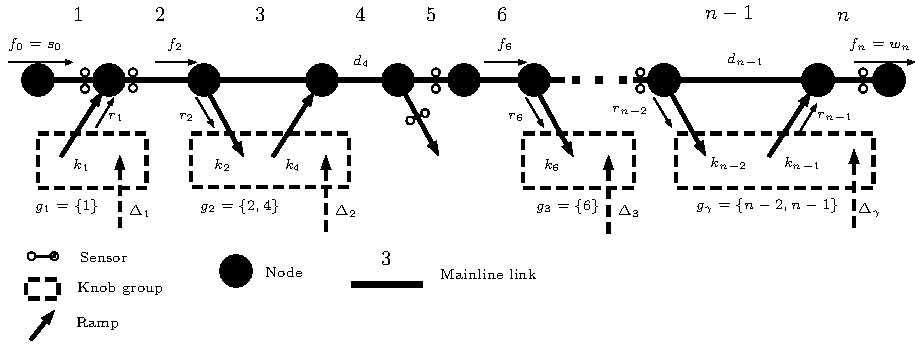
\includegraphics[width=7in]{figures/scheme.pdf}
%	\normalsize{
%		\begin{tabular}{llll}
%		\ \ \ \ \ \ \ \ \ \ \ \ \ \ && \ \ \ \ \ \ \ \ \ \ \ \ \ \ & \\ 
%
%			&$M=\llbracket 1,n \rrbracket$ && Mainline links indexes\\
%			&$S=\{ i_{1},i_{2},...,i_{s}\}\subset{M\cup\{0\}}$ && Source links indexes (index of preceding 	mainline link)\\
%			&$W=\{ i_{1},i_{2},...,i_{w}\}\subset{M}$ && Sink ("well") links indexes (index of preceding mainline link)\\
%			&$T=\{ i_{1},i_{2},...,i_{\mu}\}\subset{M}$ && Monitored (T for tracked) mainline links indexes\\
%			&$K=\{ i_{1},i_{2},...,i_{\kappa}\}\subset{S\cup W\backslash \{0,n\}}$ && Non-Monitored ramps indexes : the "knob ramps"\\
%			&$G=(g_{i})_{i\in{\llbracket 1,\gamma \rrbracket}}$ && Knob groups\\
%			&$k_{p}=(k_{i_{1}}^{(p)},k_{i_{2}}^{(p)}...,k_{i{\kappa}}^{(p)})$ && Knobs value vector at iteration p\\
%			&$\sigma=(\sigma_{i_{1}},\sigma_{i_{2}}...,\sigma_{i_{\kappa}})$ && $\pm1$ : on- or off-ramp indicator for knobs\\
%			&$(L_{i})_{i\in M}$ && Mainline link lenghts\\
%			&$(f^{(p)}_{i}(t))_{i\in{M}}$ && Mainline out flows at iteration p\\
%			&$(s^{(p)}_{i}(t))_{i\in{S}}$ && Source out flows at iteration p\\
%			&$(w^{(p)}_{i}(t))_{i\in{W}}$ && Sink out flows at iteration p\\
%			\\
%		\end{tabular}
%	}
	\rule{7in}{0.3pt}
	\caption{Freeway model and notation}
	\label{fig:scheme}
\end{figure*}

\label{subsubsec:freeway_notation}
\subsubsection{Traffic model}
\label{subsubsec:traffic_notation}
$\forall t \in \tau,\ (f_{i}(t))_{i\in{M}}$ and $(r_{i}(t))_{i\in{R}}$ are the flows exiting respectively the mainline and ramp links at time $t$, output by the model.\\
In addition, $f_{0}(t)$ is the flow entering the first mainline link (entrance of the freeway).\\
$\forall t \in \tau,\ (d_{i}(t))_{i\in{M}} $ are the densities on the mainline links, output by the model.\\
$\forall t \in \tau,\ \big\{\bar{f_{0}}(t) ; (\bar{r_{i}}(t))_{i\in{M}} \big\} $ are the exit flow demands imputed to the model.\\
\subsubsection{Data}
\label{subsubsec:data_notation}
\emph{As a common pattern, the measured values will be denoted with a tilde.}\\
\\
Measured mainline exit flows are denoted $(\widetilde{f_{i}}(t))_{i\in{T}}$\\
Measured mainline densities are denoted $(\widetilde{d_{i}}(t))_{i\in{T}}$\\
Measured ramp exit flows are denoted $(\widetilde{r_{i}}(t))_{i\in{(R\backslash K)}}$\\
\\
Fig.	 \ref{fig:scheme} summarizes the model. The missing notation will be introduced progressively. \\





\section{Uncertainty}
\label{sec:uncertainty}
Our problem involves three sources of uncertainty or inexactness:
\begin{itemize}
	\item Uncertainty on the data: the measurements have a certain confidence interval.
	\item Inexactness of the model itself.\\
	This inexactness reflects the fact that, even if we had perfect data and the demand on every ramp, the model would not output the exact real traffic (and congestion phenomena etc.).
	\item Inexactness of the shapes of the templates, that forces us to give freedom to the parameters.
\end{itemize}
These uncertainties and inexactness are merged into two uncertainties:
\begin{itemize}
	\item \emph{Uncertainty on the local flow measurements:} This describes the uncertainty at the link level. It is applied to the sum of all the flow measurements of one sensor during the duration.\\
	Denoting $F_{i}=\sum\limits_{t\in\tau}f_{i}(t)$ and $\widetilde{F_{i}}=\sum\limits_{t\in\tau}\widetilde{f_{i}}(t)$, this local uncertainty is divided into two competing components:
	\begin{itemize}
		\item \emph{additive local uncertainty}: denoted $U^{add}$. The additive confidence interval for $F_{i}$ is:
		\begin{equation*}
			F_{i}\in\big[\widetilde{F_{i}}-U^{add},\ \widetilde{F_{i}}+U^{add}\big]
		\end{equation*}		
		\item \emph{multiplicative local uncertainty}: denoted $U^{mul}$. The multiplicative confidence interval for $F_{i}$ is:
		\begin{equation*}
		 	F_{i}\in\big[\widetilde{F_{i}}.(1-U^{mul}),\ \widetilde{F_{i}}.(1+U^{mul})\big]
		\end{equation*}
	\end{itemize}
	\item \emph{Uncertainty on the global duration-long measurements}: This describes the uncertainty at the whole mainline level. It is a generic multiplicative uncertainty applied to all quantities that are computed from the measurements on every mainline sensor and during the whole duration. We denote this uncertainty $U^{global}$.\\
\\
Let $\widetilde{q_{i}}(t)$ a quantity computed from the measurements on link $i$ at time $t$. Denoting $Q=\sum\limits_{i\in T}\sum\limits_{t\in\tau}q_{i}(t)$ and $\widetilde{Q}=\sum\limits_{i\in T}\sum\limits_{t\in\tau}\widetilde{q_{i}}(t)$, the global confidence interval for this quantity is:\\
	\begin{equation*}
		 Q\in \big[\widetilde{Q}.(1-U^{global}),\ \widetilde{Q}.(1+U^{global})\big]
	\end{equation*}	
\end{itemize}
The reader will understand better the form chosen for the uncertainty further on.


\section{Problem formulation}
\subsection{Introduction}
\label{subsec:problem_formulation_intro}
For every monitored source or off-ramp, we input to the model the measured flow as exit flow demand.\\ The assumptions made in \ref{subsec:traffic_model} imply that this demand is approximately equal to the actual model-output flow going through the ramp, for all times and above mentioned links:\\
\begin{equation}
	\label{eq:noqueue}
	\forall i\in R\backslash K,\ \forall t\in \tau,\ \widetilde{r_{i}}(t)=\bar{r_{i}}(t)\approx {r_{i}}(t)\\
\end{equation}
Therefore, the only missing parameters to the model are the flow demand profiles of the non-monitored ramps: $(\bar{r_{i}}(t))_{\stackrel{i\in K}{t \in{\tau}}}$.
Our method consists in mapping these $\kappa$ flow profiles into one parameter each.\\
To do that, a flow profile called \emph{template} is built for every non-monitored ramp. These templates, denoted $(t_{i}(t))_{\stackrel{i\in{K}}{t \in{\tau}}}$, consist in a normalized flow profile: a flow value is given to each element of $\tau$ and the resulting profile is normalized to a reasonable value $\Theta$.
For each of the non-monitored ramps $i$, we define a multiplicative factor $k_{i}$ called \emph{knob} that will set the intensity of the template. 
That is, we input as exit flow demand of the ramp its corresponding template multiplied by the ramp knob : $k_{i}.t_{i}(t)$.\\
\\
The parameters of our imputation problem are therefore the \textbf{$\kappa$ knobs}, corresponding to the $\kappa$ non-monitored ramps.\\
\\
In addition, due the same assumptions that gave Eq. \ref{eq:noqueue}, we have :\\
\\
$\forall i \in K,\ \forall t\in \tau,\ k_{i}.t_{i}(t)=\bar{r_{i}}(t)\approx r_{i}(t)$\\
\\
$and,\ especially, with\ \Theta=\sum\limits_{t\in\tau}t_{i}(t):$\\
\\
\begin{equation}
	\label{eq:noqueuetemplate}
	\sum\limits_{t \in \tau} r_{i}(t)=k_{i}.\Theta\\
\end{equation}
\subsection{Constraints on the parameters}
\label{subsec:constraintsintro}
We define here the constraints verified by the knobs. They consist in box hard boundaries and linear inequalities.
\\
\emph{Notation:}\\
\\
$\vec{k}=(k_{i_{1}},k_{i_{2}},...,k_{i{\kappa}})$ is the vector containing the value of the knobs.\\
$\sigma=(\sigma_{i_{1}},\sigma_{i_{2}},...,\sigma_{i_{\kappa}})$ is the source/sink indicator vector for the knobs: \\
\\
$\forall j\in{K}, \ \sigma_{j}=\bigg\{$
\begin{tabular}{l}
	$1\ if\ j\in{S}$ \\
	$-1\ if\ j\in{W}$ \\
\end{tabular}\\
\\
For clarity, we will often abusively use the expression \emph{knob i} or \emph{knob-ramp i} instead of \emph{ramp corresponding to the knob i}.
\subsubsection{Physical boundaries}
\label{subsubsec:naive}
The box constraints applied to each knob are physical capacity limits imposed by the ramp they are associated with. They reflect that the maximum value of the ramp flow cannot exceed the capacity of the ramp.\\
\\
\begin{tabular}{l}
	$\forall i\in{K}$, the maximum $m_{i}$ of knob $i$ is defined by:
	\\
	\\
	$\forall t \in \tau,\ k_{i}.t_{i}(t)\bar{r_{i}}(t)\leq\ \scriptstyle{[Capacity\ of\ the\ ramp\ associated\ to\ knob\ i]}$
	\\
	\\
	$\Rightarrow m_{i}=\frac{[Capacity\ of\ the\ ramp\ associated\ to\ knob\ i]}{\max_{t} t_{i}(t)}$\\
	\\
	\\
	$therefore:$ \\
	\\
	$\forall i\in{K},\forall p\in{\mathbb{N}},\ 0\leq k_{i}\leq m_{i}$\\
	\\
	$\Leftrightarrow  \vec{0}\leq \vec{k}\leq \vec{m},\ with\ \vec{m} =\begin{bmatrix}m_{1}\\m_{2}\\\vdots\\m_{\kappa}\end{bmatrix}$\\
	\color{red}Define $\leq$ for vectors ?\\
	 \color{red}Define these boundaries as a box $B$ ?\color{black}
\end{tabular}




	
\subsubsection{Knob groups and flow balance}
\label{subsubsec:knob_groups}
We define here objects and notation to describe a simple situation: the knobs are closely monitored by nearby mainline sensors, leading often to a situation where a ramp is the only non-monitored ramp between two mainline sensors. This is equivalent to it being monitored, if it was not for the uncertainties.\\
\\
We call \emph{segment} the set of links between two consecutive mainline sensors, including the links containing these sensors. \\
We call \emph{knob group} each set of knobs whose corresponding ramp is connected to the same monitored segment.
This definition is illustrated in Fig. \ref{fig:scheme}.\\
We call \emph{partially monitored segment} the monitored segments associated with a knob group i.e. containing at least one non-monitored ramp.\\
\\
Denoting $\gamma$ the total number of knob groups, we have:\\
\\
$Partially\ monitored\ segments:\ (S_{i})_{i \in \llbracket 1,\gamma \rrbracket}$\\ 
\\
Formal definition:\\
$\exists\ !\ \gamma\in M,\ \exists\ !\ ((\beta_{i},\eta_{i}))_{i\in\llbracket 1,\gamma\rrbracket}\in (T^2)^{\llbracket 1,\gamma\rrbracket}\ s.t.,$\\
$denoting\ S_{i}=\llbracket \beta_{i},\eta_{i} \rrbracket\ and\ S=\underset{i\in \llbracket 1,\gamma \rrbracket}{\bigcup}  S_{i}:$\\
$\forall i\in\llbracket 1,\gamma \rrbracket,$
\begin{enumerate}
	\item $\llbracket \beta_{i},\eta_{i} \rrbracket \cap T=\{\beta_{i},\eta_{i}\}$
	\item $\llbracket \beta_{i}, \eta_{i} \rrbracket \cap K\not= \{\emptyset \}$
\end{enumerate}
$and\ \forall k\in K, k\in S.$\\
\\
and\\
\\
$Knob\ groups:\ (g_{i})_{i\in \llbracket 1,\gamma \rrbracket}$\\
\\
Formal definition:\\
$\forall i \in \llbracket 1, \gamma \rrbracket,\ g_{i}=\llbracket \beta_{i}, \eta_{i} \rrbracket \cap K $\\
\\
We can deduce the value of the daily flow brought by the knobs of each group from the \emph{knob group flow balance}: the difference between all the flows entering and all the flows exiting their incomplete monitored segment. That is the sum of the flow exiting the mainline entrance of the segment and the flows exiting the monitored on-ramps throughout the segment minus the sum of the flow exiting the mainline exit of the segment and the flows exiting the monitored off-ramps throughout the segment. \\ 
\color{red}Put here the paragraph Gabriel wrote\color{black}\\
\\
$Knob\ group\ flow\ balances:\ (\Delta_{i})_{i\in \llbracket 1,\gamma \rrbracket} $\\
\\
Formal definition:\\
$\forall i \in \llbracket 1,\gamma \rrbracket,\ \forall t\in \tau,$\\
$\Delta_{i} =$\small $\mathlarger{\sum\limits_{t\in \tau}}\bigg[\widetilde{f}_{\beta_{i}}(t)-\widetilde{f}_{\eta_{i}}(t)+\sum\limits_{j\in (R\backslash K)\cap S_{i}}\sigma_{i}.\widetilde{r_{j}}(t)\bigg]$\normalsize 
\\
\\
\\
The balance equation of each partially monitored segment is:\\
\\
$0=\mathlarger{\sum\limits_{t\in \tau}}\bigg[f_{\beta_{i}}(t)-f_{\eta_{i}}(t)+\sum\limits_{j\in R\cap S_{i}}\sigma_{i}.r_{j}(t)\bigg]$\\
\\
As stated in eq. \ref{eq:noqueue}, the model-output flows exiting the ramps are equal to their demand flows. The balance equation becomes therefore:\\
\\
$0=\Delta_{i}+\mathlarger{\sum\limits_{t\in \tau}}\bigg[\sum\limits_{j\in K\cap S_{i}}\sigma_{i}.r_{j}(t)\bigg]$\\
\\
Leading to:\\
\\
$\Delta_{i}=\mathlarger{-\sum\limits_{t\in \tau}}\bigg[\sum\limits_{j\in K\cap S_{i}}r_{j}(t)\bigg]$\\
\\
$\Leftrightarrow \Delta_{i}=\mathlarger{-\sum\limits_{j\in K\cap S_{i}}}\sigma_{i}\bigg[\sum\limits_{t\in \tau}r_{j}(t)\bigg]$\\
\\ 
and thanks to eq. \ref{eq:noqueuetemplate}:
\begin{equation}
\centering
\label{eq:balance}
\Leftrightarrow\ \ \Delta_{i}=-\sum\limits_{j\in K\cap S_{i}}\sigma_{j}.k_{j}.\Theta
\end{equation}
Eq. \ref{eq:balance} shows that, for every knob group, the knobs composing it are linked by one linear equation.\\
This equation determines uniquely the value of the single-knob groups and links the multiple-knob groups with one linear constraint. The next paragraph describes how we apply uncertainties to this equation in order to produce new, closer to reality knob boundaries.\\


\subsubsection{Refined knob boundaries}
\label{subsubsec:refined}
The local uncertainty described in \ref{sec:uncertainty} prevents us from keeping Eq. \ref{eq:balance} as a constraint for the parameters.\\
\\
$\forall i \in {\llbracket 1,\gamma \rrbracket}$, let the most permissive boundaries:\\
\\
$\Delta_{i}^{-}=\min{\{|\Delta_{i}|-U^{add};|\Delta_{i}|.(1-U^{mul})\}}$\\
$\Delta_{i}^{+}=\max{\{|\Delta_{i}|+U^{add};|\Delta_{i}|.(1+U^{mul})\}}$\\
\\
Taking the local uncertainty into account in Eq. \ref{eq:balance} is translated into the following linear inequality constraints:\\
\begin{equation}
\label{eq:ineq}
	\forall i\in \llbracket 1,\gamma \rrbracket,\ \Delta_{i}^{-}\leq |\sum\limits_{j\in g_{i}}\sigma_{j}.k_{j}.\Theta| \leq \Delta_{i}^{+}
\end{equation}
\\
These $\gamma$ inequalities drastically reduce the size of the search space, defining a new \emph{feasible space}.\\
\\
\emph{Comments:}\\
We can now illustrate and justify the form that we have adopted for the uncertainty. This form allows us to quantify the freedom given to the result: the flow balance of each knob-group is between $(1-U^{mul})$ and $(1+U^{mul})$ times what has been measured by the mainline sensors, aknowledging that we don't accept less than $\pm U^{add}$ cars precision on the measures.\\
Taking into account $U^{add}$ is indispensable. This is observed in the case of single-knob groups, where Eq. \ref{eq:balance} leads to a unique value for the knob of the group. Let us call it \emph{perfect value of the knob i}, denoted $k_{i}^{perfect}$. If $U^{add}=0$, it immediately follows from Eq. \ref{eq:ineq} that two new boundaries are set for $k_{i}$, if they are tighter than $[0,m_{i}]$ : $k_{i}\in [(1\pm U^{mul}).k_{i}^{perfect}]$.\\
The problem happens when the perfect value is a ridiculously small quantity. The maximum obtained with $(1+ U^{mul}).k_{i}^{perfect}$ then corresponds often to a total daily flow of less than $500$ cars exiting the ramp, which is not acceptable.\\ 
\\
\emph{Example:} In the scenario we experiment on, one of the ramps has a perfect value of $0.016$, which leads to a maximum of $0.032$ i.e. $406$ cars going through the ramp during the whole day if $U^{mul}$ is set to $100\%$ (very permissive: the daily flow can double what is measured by the mainline sensors). This is way too small for the scenario.\\ 
However, in fact, the fluctuation allowed by the new boundaries of this ramp is $406\ cars$, which is $13$ times smaller than the sensor uncertainty (i.e. $5 \% .[mean\ on\ i\in T\ of\ \widetilde{F_{i}}]=5139\ cars$): the sensors do not have this level of precision, and the sensor noise/bias is responsible for this impossible perfect value. \\
Once $U^{add}=5\%.[mean\ on\ i\in T\ of\ \widetilde{F_{i}}]$ is taken into account, the maximum of the knob becomes $0.42$, which corresponds to $5329\ cars$  and offers an acceptable range to the flow going through the ramp.\\
\color{red}THIS IS WHERE IVE STOPPED WORKING TODAY\color{black}
\subsection{Performance calculators}
\label{subsec:pcs}
Three performance calculators (PC) are used for the error calculation:
\color{red}\emph{We describe here qualitatively the performance calculators themselves, not the error calculation (that's why I mention congestion and not congestion pattern fitting).}\color{black}
\begin{itemize}
	\item \emph{Vehicle miles traveled} (VMT): sum of the distance travelled on the mainline by each car, over the whole day. \emph{Explain why it is important in traffic study, why we have chosen it} 
	\item \emph{Vehicle hours traveled} (VHT): sum of the time spent on the mainline by each car, over the whole day. \emph{explain why it is important in traffic study, why we have chosen it} 
	\item \emph{Congestion}: according to \emph{blabla} theory, we define the congested links as the links where the density exceeds the \emph{critical density} defined by the link's fundamental diagram. The main feature of our method is to fit the locations and times of these congested links to what the measurements indicate.
\emph{explain why we have chosen it}
\end{itemize}

\subsection{Fitness function}
\label{fitnessintro}
The calibration method consists in minimizing jointly the three errors described in \ref{subsec:pcs_intro}. We accomplish this goal by minimizing an \emph{objective function} $\Phi$, which is the weighted sum of the errors modified by the global uncertainty, as explained below.\\
\\
\emph{Uncertainty handling :} $U^{global}$, described in \ref{subsec:data}, defines a tolerance threshold for the error results. The error results below $U^{global}$ are set to zero, in order to avoid any discrimination between them (we do not have a level of precision below $U^{global}$).\\
Each of the three errors $E$ will therefore be multiplied by $\mathds{1}_{(E>U^{global})}.$\\ 
\\
Let $(w_{i})_{i\in\llbracket 1,3 \rrbracket}$ the weights, verifying :\\
$w_{1}+w_{2}+w_{3}=1\ and\ \forall i\in \{1,2,3\},\ w_{i}\geq 0.$\\
\\
Let the three error \emph{contributions}:\\
$\phi_{VHT}(\vec{k})=w_{1}.E_{VHT}(\vec{k}).\mathds{1}_{(E_{VHT}>U^{global})}$\\
$\phi_{VMT}(\vec{k})=w_{2}.E_{VMT}(\vec{k}).\mathds{1}_{(E_{VMT}>U^{global})}$\\
$\phi_{CP}(\vec{k})=w_{3}.E_{CP}(\vec{k}).\mathds{1}_{(E_{CP}>U^{global})}$\\
\\
$\Phi$ is defined by:\\
\begin{displaymath}
		\Phi:
		\left|
  		\begin{array}{rcl}
    	\mathscr{B} & \longrightarrow &[0,100] \\
    	\vec{k} & \longmapsto &  \phi_{VHT}(\vec{k})+\phi_{VMT}(\vec{k})+\phi_{CP}(\vec{k}) \\
  	\end{array}
	\right.
\end{displaymath}
\\
\emph{Note : the errors can lead to values superior to 1 thus giving values of $\Phi$ superior to 100\% but, to simplify, we will ignore these cases that are very far from the objective.}\\
\\

This definition as a weighted sum of percentages implies that the values of $\Phi$ can be interpreted as a \emph{global error percentage}. Thanks to the normalization of the errors, the weight given to each component is equivalent to the importance the operator wants to give to each one of them.

\subsubsection{Total Vehicle Miles}
\label{subsubsec:tvm}
This quantity is the sum of the distance traveled on the mainline by each car, over the whole duration.
Obviously, it is computed using only the monitored mainline links, for the comparison with the data to be relevant.
\color{red}Explain why it is important in traffic study, why we have chosen it\color{black}
\\
VMT computation on monitored mainline links output and data:
\begin{equation*}
	 VMT(\vec{k})=\sum_{i\in{T}}L_{i}\sum_{t\in \tau}f_{i}(t)
\end{equation*}
\\
Denoting $\widetilde{VMT}$ the value computed from the data using the same formula, the error is the relative difference :\\
\\
\begin{equation*}
	E_{VMT}(\vec{k})=\frac{|VMT(\vec{k})-\widetilde{VMT}|}{\widetilde{VMT}}
\end{equation*}

\emph{Reduction of the feasible space:} we present here a method used to reduce the feasible space size by forcing the knobs to match the correct VMT value.\\
VMT is the result of a simple \emph{a priori} calculation that does not need the traffic model output calculation, if we know the boundary conditions at $t=0$ and $t=D$. As exposed in \ref{subsec:model}, we assume that these conditions are $0\ cars$ on every link ($D$ has to be big enough for these conditions to be very small in comparison with the total number of vehicles during $D$).\\
\\
Let $VMT^{ref}=VMT(\vec{k}^{ref})$, a certain $VMT$ reference value output by the model. We suppose that $\vec{k}^{ref}$ is some feasible knobs vector (in our case, we used $\vec{k}^{ref}=(1,...,1)$).\\
Denoting $VMT^{a priori}(\vec{k})$ the expected VMT value computed from $\vec{k}$:\\
\begin{equation}
	\label{eq:TVMapriori}
	VMT^{a\ priori}(\vec{k})=VMT^{ref}+\mathlarger{\sum\limits_{i\in K}}\biggl[\sigma_{i}.k_{i}.\Theta.	\sum\limits_{\underset{j>i}{j\in T}}L_{j}\biggr]
\end{equation}	
The \emph{a-priori} calculation above relies on anticipating the changes from $VMT^{ref}$ caused by changing the knobs from $\vec{k^{ref}}$ to $\vec{k}$. For each knob, the flow change resulting from its modification is multiplied by the remaining mainline length and the "on/off-ramp indicator". All these contributions are then summed.\\
\\
The linear equation \ref{eq:TVMapriori} empowers us to constrain the input $\vec{k}$ in order to ensure $VMT(\vec{k})\approx \widetilde{VMT}$, thus reducing the size of the feasible space by one dimension:
\begin{equation*}
	\mathlarger{\sum\limits_{i\in K}}\biggl[\sigma_{i}.k_{i}.\Theta.	\sum\limits_{\underset{j>i}{j\in T}}L_{j}\biggr]=\widetilde{VMT}-VMT^{ref}
\end{equation*}
However, the global uncertainty applied on TVM (which is a global quantity computed from the sum over the whole time and space) forces us to loosen this constraint equation.\\
Denoting $\widetilde{VMT}^{-}=\widetilde{VMT}.(1-U^{global})$ and\\ $\widetilde{VMT}^{+}=\widetilde{VMT}.(1+U^{global})$, it becomes:\\
\begin{equation}	
	\label{eq:TVMineq}
	\widetilde{VMT}^{-}\leq\mathlarger{\sum\limits_{i\in K}}\biggl[\sigma_{i}.k_{i}.\Theta.	\sum\limits_{\underset{j>i}{j\in T}}L_{j}\biggr]+VMT^{ref}\leq \widetilde{VMT}^{+}
\end{equation} 
\subsubsection{Total Vehicle Hours}
\label{subsubsec:tvh}
This quantity is the sum of the time spent on the mainline by each car, over the whole duration.
Obviously, it is computed using only the monitored mainline links, for the comparison with the data to be relevant.\\
\\
VHT computation on monitored mainline links output:
\begin{equation*}
	 VHT(\vec{k})=\frac{dt}{[1\ hour]}\sum_{i\in{T}}L_{i}\sum_{t\in \tau}d_{i}(t)
\end{equation*}
\\
Denoting $\widetilde{VHT}$ the value computed from the data using the same formula, the error is the relative difference :
\begin{equation*}
	E_{VHT}(\vec{k})=\frac{|VHT(\vec{k})-\widetilde{VHT}|}{\widetilde{VHT}}
\end{equation*}
~\\
\subsubsection{Congestion Pattern}
\label{subsubsec:cp}
We call \emph{contour plot} the graph representing the value of a quantity on every mainline link at all times: the mainline links as absciss and time steps as ordinates.
Fig. \ref{fig:beats_contour}. below is an example of a density contour plot for one day on a 135 links freeway, from a traffic model output.\\
\begin{figure}[h]
	\centering
	\label{fig:beats_contour}
	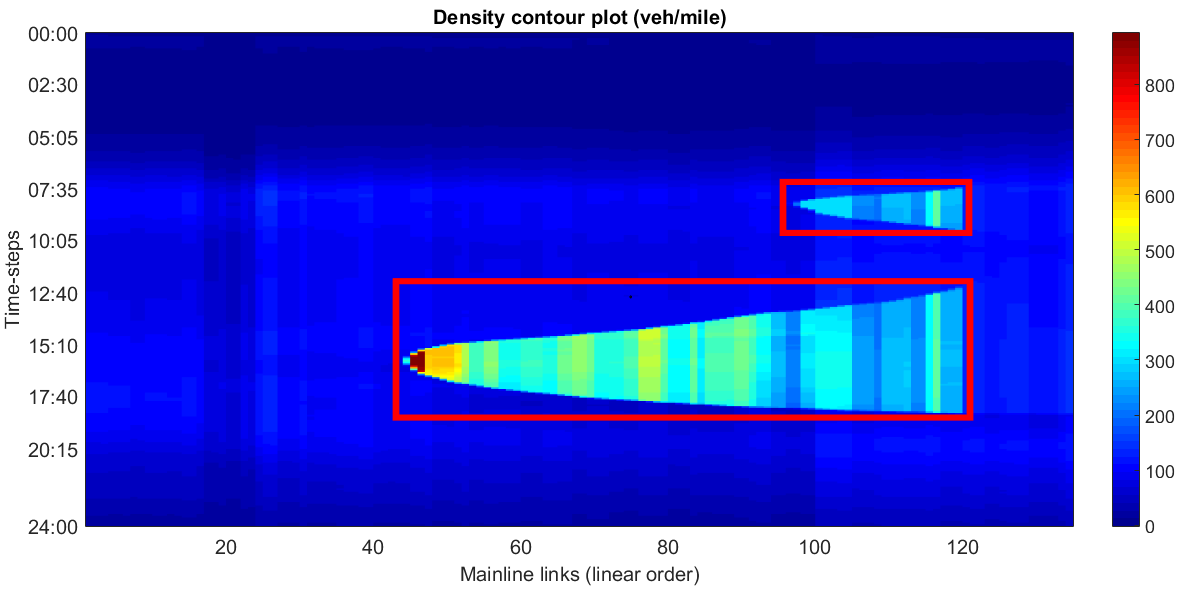
\includegraphics[width=7in]{beats_contour.png}
	\caption{Example of a density contour plot on a 135 mainline links freeway over 24h out of a traffic model output.}
\end{figure}
This plot is used to monitor easily where and when the congestion is : here, we see empirically that it is contained in the two framed parts.\\
In what follows, by analogy, we will call \emph{contour domain} the set $\mathscr{P}$=$\big\{(i,t)|\ i\in M,\ t\in\tau\big\}$ and \emph{pixel} each of its elements.\\
On the model output, we define the \emph{congested} pixels as the ones where the density exceeds some \emph{critical density} deduced for each link from the freeway and traffic models. The main feature of our calibration method is to fit the locations and times of these congested pixels to what the measurements indicate.\\
For each mainline link $i\in{M}$, we denote $d_{i}^{*}$ the critical density.
\\
We define the \emph{output congested domain} $\mathscr{C}\in\mathscr{P}$ containing the congested pixels :
\begin{equation*}
	\mathscr{C}=\big\{ (i,t)\in{\mathscr{P}}\ |\ {d_{i}(t) \geq d_{i}^{*}}\big\}
\end{equation*}
%We also define the \emph{congestion pattern} performance metric $CP$ as the signaling matrix 
%of $\mathscr{C}$ :
%\begin{equation*}
%	CP=\big(\mathds{1}_{(i,j.dt)\in \mathscr{C}}\big)_{\stackrel{i\in M}{j\in \llbracket 0,\frac{D}{dt}\rrbracket}}
%\end{equation*}
To define an error based on $\mathscr{C}$, a domain supposed to contain the congestion as to be determined.
From the data \emph{density contour plot} (partial, obtained only on the monitored links), we define a domain $\widetilde{\mathscr{C}}\subset\mathscr{P}$ fitting the congested pixels as best as it can following some criteria (how this domain is built depends on the amount of data the operator possesses and on his goals. In our case, $\widetilde{\mathscr{C}}$ was a set of rectangles containing all the congestion seen in the data contour plot).\\
%The same way we defined $CP$, we define $\widetilde(CP)$ as the signaling matrix of $\widetilde{C}$:
%\begin{equation*}
%	\widetilde{CP}=\big(\mathds{1}_{(i,j.dt)\in \mathscr{\widetilde{C}}\big)_{\stackrel{i\in M}{j\in \llbracket 0,\frac{D}{dt}\rrbracket}}
%\end{equation*}
\\
We can now define the congestion pattern error denoted $E_{CP}$ as the normalized number of wrong congestion state pixels. That is, we add one to $E_{CP}$ for each pixel that is not congested but should and for each pixel that is congested but shouldn't. We then divide this result by the number of pixels that should be congested (i.e. $Card(\widetilde{\mathscr{C}})=\sum_{t\in{\tau}}\sum_{i\in{M}}\mathds{1}_{(i,t)\in{\widetilde{\mathscr{C}}}}$).
\begin{equation*}
	E_{CP}(\vec{k})=\frac{\sum_{t\in{\tau}}\sum_{i\in{M}}\mathds{1}_{\{(i,t)\in{(\widetilde{\mathscr{C}}\backslash \mathscr{C})\cup(\mathscr{C}\backslash \widetilde{\mathscr{C}} })\}}}{\sum_{t\in{\tau}}\sum_{i\in{M}}\mathds{1}_{(i,t)\in{\widetilde{\mathscr{C}}}}}
\end{equation*}
Note that $E_{CP}$ becomes very sensible if the data does not contain much congestion (i.e. $Card(\widetilde{\mathscr{C}})<<Card(\mathscr{P})$).\\
\\
Fig. \ref{fig:cp_example}. below is a visual representation on a contour domain of $(\widetilde{\mathscr{C}}\backslash \mathscr{C})$ otherwise called \emph{false negative pixels}, $(\mathscr{C}\backslash\widetilde{\mathscr{C}})$ otherwise called \emph{false positive pixels} and $(\mathscr{C}\cap\widetilde{\mathscr{C}})\cup \big(\mathscr{P}\backslash(\mathscr{C}\cup \widetilde{\mathscr{C}})\big)$, which are the \emph{correct congestion matching} pixels. 
\\Here, $\widetilde{\mathscr{C}}$ is the yellow rectangle.
\begin{figure}[h]
	\caption{Visual example of the congestion pattern matching computation. $\widetilde{\mathscr{C}}$ is one rectangle.}
	\label{fig:cp_example}
	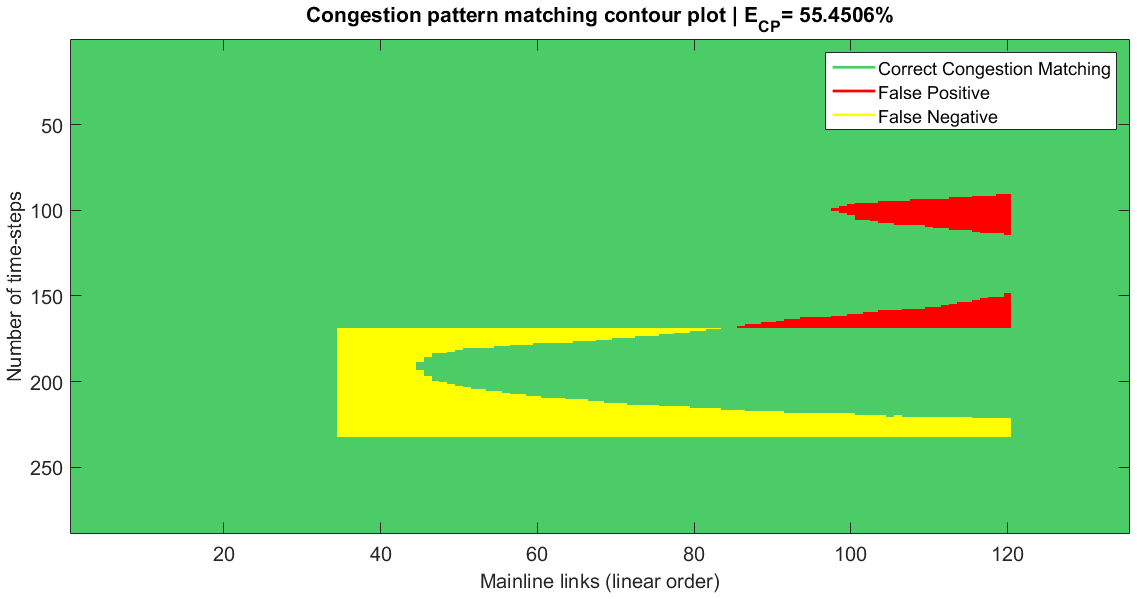
\includegraphics[width=7in]{figures/cp_example.png}
\end{figure}

\subsubsection{Optimization problem statement}
\label{subsubsec:statement}
enter statement here


\section{Numerical method}
\subsection{Requirements}
\label{subsec:requirements}
%\color{red}{\emph{Keywords and ideas: non-convex, ruggued search landscape(i.e.:sharp bends, discontinuities, outliers, noise, local optima), badly scaled and/or highly non-separable, convergence, adaptive, Black-Box, evaluated search points are the only accessible information on f, Randomized/stochastic works well, Robust, imputation, continuous domain.}}
%\color{black}

The performance errors are irregular functions. In particular, the congestion pattern fitting reflects congestion phenomena. These present numerous thresholds in their non-smooth behavior.\\
We can also point out that these errors aren't always correlated.\\
Furthermore, each evaluation of the error function requires the execution of a simulation (around 5 seconds on a desktop computer), and this evaluation is the only thing accessible of $\Phi$: there is no way of quickly computing its value or its gradient .\\
Therefore, the objective function is a black box.\\
We deduce from these observations that convex optimization methods and derivative-based methods are not adapted to our case.\\
The search space is a continuous hyper-cube, as explained in \ref{subsubsec:naive}.\\
We can conclude that we study a non-linear, non-convex black-box imputation problem in continuous domain.\\
\\ 	
In addition, the resolution method has to be adaptive, since it will be applied to many different freeways, times and sensor densities. We want as few numerical method parameters to tune as possible and  no prior optimization knowledge required if possible.\\
\\
%	\item What kind of algorithm is suitable
Finally, our approach does not take execution time as a criteria : the goal is to obtain the best possible result quality and uniqueness (global minimum of $\Phi$).

\subsection{Co-variance Matrix Adaptation - Evolution Strategy (CMA-ES)}
\label{subsec:cmaes}
Talk about CMAES characteristics and why it is very well suited for this.\\
\color{red}\emph{Most of the stuff will come from :}
\begin{itemize}
	\item https://www.lri.fr/~hansen/cmaesintro.html
	\item https://www.lri.fr/~hansen/cmatutorial.pdf
	\begin{itemize}
		\item 0.3: Randomized Black-Box optimization
		\item 5: Discussion
	\end{itemize}	\color{black}

	\item explain how the sampling works
	\item Consider the search costs together with the achieved objective function value.
	\item define \emph{fitness function}
\end{itemize}
	\color{black}

\subsection{Constraints implementation}
\label{subsec:implementation}
The CMA-ES source code handles box constraints natively using the "repair and penalize" procedure. This consists in repairing non-feasible sampled points before inputting them to the model; and penalizing (i.e. increasing the value of the fitness function) proportionally to the distance between the unfeasible point and the feasible space. This method forces the algorithm to eventually enter and stay in the feasible domain while avoiding evaluating non-allowed points.\\
However, the source code does not handle linear constraints. We describe here how we apply manually this repair \& penalize procedure to reflect the two linear constraints shown in \ref{subsec:statement}.\\
\newpage
\emph{Repairing:}\\
\\
Let $\underline{\vec{k}}^{(p)}$ the knobs vector sampled by CMA-ES at iteration $p$ (i.e. before repairment).\\
The projection is implemented using the following program in a standard quadratic optimization solver:\\
\\
$minimize \ \ \ \ \ \ \norm{\vec{k}^{(p)}-\underline{\vec{k}}^{(p)}}_{2}$\\
$s.t.\ \ \ \forall i\in{G}, \ \ \Delta_{i}^{-}< |\sum_{j\in{g_{i}}} \sigma_{j}.k_{j}.\Theta|<\Delta_{i}^{+}$\\
$and\ \widetilde{VMT}^{-}\leq\mathlarger{\sum\limits_{i\in K}}\biggl[\sigma_{i}.k_{i}.\Theta.	\sum\limits_{\underset{j>i}{j\in T}}L_{j}\biggr]+VMT^{ref}\leq \widetilde{VMT}^{+}\nonumber $\\
$and\ \ \ \ \vec{k}^{(p)}\in \mathscr{B}$\\
\\
Let us illustrate the effect of this program with an example. We suppose that the $\widetilde{VMT}^{\pm}$ condition above is enough loose for it to be respected without influencing the projection (often verified in practice).
\begin{figure}[h!]
\centering
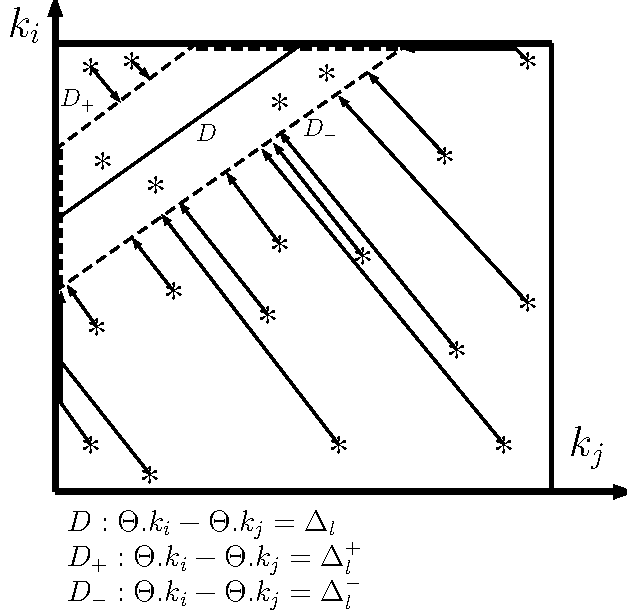
\includegraphics[width=3in]{figures/proj.pdf}
\caption{Example of repair projections on a two-knobs group.}
\label{fig:proj}
\end{figure}
Fig. \ref{fig:proj} below displays, for a two-knobs group $g_{l}=\{i,j\}$, the projection of several sampled points due to the two remaining conditions ($\Delta_{l}^{\pm}$ and $\mathscr{B}$). $D$ is the hyper-plan (straight line in dimension 2) on which the knob group flow will have the exact value $\Delta_{l}$.
The two \emph{tolerance hyper-plans} on which the knob group flow value will be $\Delta_{l}^{+}$ and $\Delta_{l}^{-}$ are respectively $D^{+}$ and $D^{-}$.
In addition, the external square is the hyper-cube corresponding to the physical boundaries of the two knobs (from $\mathscr{B}$). 
The points sampled in the feasible space (the doted line trapezium) remain untouched while the others are projected on the nearest point of the edge of the feasible space.\\
This repair ensures that only feasible values of the input are tested and that the algorithm does not get stuck in an unfeasible hole of the physical boundaries hyper-cube.\\

\emph{Penalizing:}\\
\\
At each evaluation, a penalization proportional to the distance between the projected and original point is added to the fitness function. This ensures that the algorithm will come closer to the feasible space at every iteration until eventually entering and staying inside it. This feature is important as it avoids two imbalances on the sampling:
\begin{itemize}
	\item Testing more points on the edges than we should: if the algorithm is left sampling points far from the edges, without penalization, it will have no incentive to prefer sampling next to the feasible space than far. This is an obstacle from entering the feasible space, as all the points on the straight lines perpendicular to the edges would be equivalent. This would lead to a situation where it is common that too much (or all) of the points are sampled on the edges while CMA-ES converges far from the feasible space.
	\item Imbalance between the edge points tested: the edge points which are the projection of more unfeasible hyper-cube points than others will be sampled unfairly more often.\\
	\emph{Example:} in Fig. \ref{fig:proj}, the points of the square on the mediator of the segment formed by the intersections of D and the square are more numerous than the points on any other straight with same slope.\\
The points on one of these straights and below the feasible space are all projected to the same point of the edge of the feasible space. Therefore, without penalization, the middle of the segment cited above would be sampled more often than the other points of its edge, for a reason that is not the simulation output it leads to. 
\end{itemize}
~\\
The penalization, denoted $E_{proj}$, is normalized by a factor which is the distance between the physical maximums and minimums vectors, reflecting the \emph{order of magnitude} of the search space.
\begin{equation*}
	E_{proj}(\underline{\vec{k}}^{(p)},\vec{k}^{(p)})=\frac{\norm{\vec{k}^{(p)}-\underline{\vec{k}}^{(p)}}_{2}}{\norm{\begin{bmatrix}m_{1}\\m_{2}\\\vdots\\m_{\kappa}\end{bmatrix}-\begin{bmatrix}0\\0\\\vdots\\0\end{bmatrix}}_{2}}
\end{equation*}
A fourth contribution $\phi_{proj}=w_{4}.E_{proj}(\underline{\vec{k}}^{(p)},\vec{k}^{(p)})$ is therefore added to the fitness function.\\
\\
With the same definitions as in \ref{subsec:fitnessintro} and\\
$\sum_{i=1}^{4} w_{i}=1\ and\ \forall i\in\llbracket 1,4\rrbracket\ w_{i}\geq 0$,\\
\\
the final fitness function used is $J$ defined by :\\
\begin{equation*}
		J:
		\left|
  		\begin{array}{rcl}
    	\mathscr{B} & \longrightarrow &[0,100] \\
    	\underline{\vec{k}}^{(p)} & \longmapsto &  \Phi(\vec{k}^{(p)})+w_{4}.E_{proj}(\underline{\vec{k}}^{(p)},\vec{k}^{(p)}) \\
  	\end{array}
	\right.
\end{equation*}
\\
We denote $J^{*}$ the minimum of $J$ encountered by CMA-ES during its search :
\begin{equation*}
	J^{*}=\min_{p}{J({\vec{k}^{(p)})}}
\end{equation*}
\\
Similarly, all values (input or output) denoted with stars are the ones corresponding to the $J$ evaluation that gave $J^{*}$.\\
\\
\emph{Single-knob group specificity:} For a single-knob group, the condition Eq. \ref{eq:ineq} is equivalent to hard boundaries for the concerned knob (one equation in one dimension). In this case, the projection due to Eq. \ref{eq:ineq} is not implemented but the physical boundaries (from $\mathscr{B}$) of the knob input to CMA-ES are replaced by these new boundaries, if they are narrower :\\
\\
$\forall\ i\in G\ s.t.\ Card(g_{i})=1,\ i.e.\ g_{i}=\{j\}\ :$
\begin{equation}
	\frac{\max{\big\{0;|\Delta_{i}^{-}|\big\}}}{\Theta}\leq k_{j} \leq \frac{\min{\big\{m_{j};|\Delta_{i}^{+}|\big\}}}{\Theta}
\end{equation}

\subsection{Large traffic simulator}
\label{subsec:simulator}
The macroscopic traffic simulator used is the Berkeley Advanced Traffic Simulator (BeATS). \emph{talk about BeATS in "split ratio as output" mode}\\
The inputs of the simulator are:
\begin{itemize}
	\item Fundamental Diagram of every link (4 parameters for each: \emph{capacity}, \emph{congestion speed}, \emph{free-flow speed} and \emph{jam density}).
	\item Entry flow of every source and sink. Timestep is 5 minutes, as for the data.
\end{itemize}
The outputs are the entry and exit flows, density and speed in every link.

\subsection{Context: Origin and reliability of the data}
\label{subsec:pems}
The real scenario used for this study is a portion of freeway 210 East in the suburbs of Los Angeles. The measurements used are collected by the sensors network PeMS of Caltrans. For more information, see http://pems.dot.ca.gov/\\
These daily measurements are flow, density and speed on 74 links of 188, every 5 minutes for 24 hours (289 time-steps).\\
After deleting partial or too biased data, the sensors have the following distribution:
\begin{itemize}
	\item 33/135 monitored mainline links
	\item 26/28 monitored on-ramps
	\item 15/25 monitored off-ramps
\end{itemize}
This makes a total of \textbf{12 knobs}.\\
\\
We chose to calibrate the model on the average of 5 Tuesdays (0am-12pm) in fall 2014 data. The goal is to find the set of knobs that best fits the profile of a Tuesday (the general shape of the traffic depending greatly on the day of the week).\\
\\
For each knob-ramp, the template is built by taking the average of the two closest monitored ramps that have the same size and incoming traffic context. 

\subsection{Parameters of the imputation}
\label{subsec:parameters}
In our case, the total number of parameters taken by the simulator is 12890: 4 per fundamental diagram and 289 per source and off-ramp.\\
In this experiment, the fundamental diagrams have been calibrated using Gune's algorithm \emph{talk about Gune's algorithm and the wide tolerance that allow FDS if they are more or less ~OK \color{red}(Greg said)\color{black}}.\\
For each monitored source and off-ramp, the collected entry flow data is set as input.\\
The imputation therefore lays only on the entry flows of the non-monitored ramps.\\
In order to reduce the number of variables to one per non-monitored ramp, a custom flow \emph{template} is built for each of these ramps. These templates are non-scaled daily flow profiles: each one of them as to be multiplied by a factor called \emph{knob}, in order to correspond to the the objective. \emph{talk about how the templates have been built}.

 






\section{Results}
\label{sec:results}






\begin{enumerate}
	\item Effects of changing the parameters(initial standard deviation, changing the boundaries, changing the weights, changing the uncertainty, changing size of population).
	\item Describe quality and usefulness of the result
	\item Talk about uniqueness. Way to improve (test experiment): increasing population size.\emph{Should we contact the creator of CMAES to ask him about the uniqueness of the solution (i.e. how to improve it ?}
	\item Is our problem "noisy" ?
	\item Talk about how cmaes behaves the way we want
	\item Talk about what happens when we tune also the monitored ramps knobs.	
	\item Talk about issues:
\begin{enumerate}
	\item Limit to result quality due to templates/FDS
	\item Constraints handling has to be improved because several knobs end on their boundaries values\
	\item Uncertainties are symmetric: making them fit the sensors bias (e.g. : if they always under estimate) would be better.
\end{enumerate}
	\item BLABLABLA
\end{enumerate} 


\section{Conclusion}
Calibration is one of the main concerns regarding the viability of macroscopic large traffic models. It consists in matching the reality of traffic with credible -if possible real- data, in order to be able to realize further experiments with the model (e.g. predict and quantify the decongestion effect of adding an off-ramp at some point of a freeway). In this paper, we expose a method to calibrate the missing input total daily flows, given their shape as a \emph{"template"}.\\
\\
To do so, we first formalize the calibration process as a general black-box optimization problem. We then choose a numerical method that is efficient and relevant for any problem : the powerful CMA evolution strategy.\\
We apply this numerical method to our particular freeway, large traffic simulator and template choice. The experiments show tendencies with the variation of the parameters (mainly the uncertainty). However, the inaccurate template choice, that greatly limits the best result quality, does not allow to describe deeply and accurately the effects of the parameters, especially the initial standard deviation and population size. \\
\\
This paper is a report on the advancement of a work that is much wider. It will allow to calibrate jointly all the parameters of large traffic models and will be applicable to any of such, with any scenario.

\section{deprecated paragraphs}
If a group is single-knob, then the knob value is uniquely determined by this principle. We will call it \emph{perfect value} of the knob.\\
If, on the contrary, it is a multiple-knob group, then the knobs of the group are linked by one linear equation. That is: their values are on a hyperplan of the space formed by their value as coordinates in an orthonormal base.\\
\\
An uncertainty must be introduced on these flow demands due to the inexactness of both the templates and the simulator in general. This uncertainty consists in two multiplicative factors applied to the knob group flow demands. We call them \emph{under-evaluation tolerance coefficient} and \emph{over-evaluation tolerance coefficient}, denoted respectively $\lambda$ and $\Lambda$.\emph{ see if we unify these two factors in one unique symmetric uncertainty}\\
A different uncertainty on the flow demands called \emph{local uncertainty} has been introduced in \ref{subsec:data}. As a remainder, it is caused by the uncertainty and bias on the measurements of the sensors. This uncertainty consists on a confidence interval centered in the value of the flow demand. We denote this local uncertainty $I^{local}$.
As we will see just below, these two uncertainties compete to ensure a minimum width for the knob boundaries.
\\
\\
\\
\\
\\
\color{red} Consider deleting this subsection and unifying the single-knob and multiple-knob groups into one unique description. There would be no need for perfect values, the single-knob group would be a particular case where no projection is needed.\\\color{black}
\\
\\
\normalsize
Defined only for single-knob groups, the \emph{knob perfect values} are equal to the value of the corresponding knob group flow demand divided by the sum of the knobs template, in order to ensure that the flow going trough the corresponding ramp corresponds exactly to the flow demand.\\ 
\\
\emph{Notation:}\\
\\
$Knob\ perfect\ values:\ (k^*_{i})_{i\in P}$\\
$with\ P=\big\{i\in K\ |\ \exists g\in G\ s.t.\ g=\{i\}\big\}$\\
\\
The perfect values are computed as follows, using that the total daily flow going trough a knob-ramp is the value of its knob times the sum of its template:\\
\\
$\forall i \in P,\ given\ j\ s.t.\ \ g_{j}=\{i\}\ and\ T_{i}=\sum_{t=0}^{24h} t_{i}(t)\ :$\\
\begin{equation*}
	\centering
	k^{*}_{i}=\frac{\Delta_{j}}{T_{i}}\
\end{equation*}
The boundaries of the knobs of single-knob groups are refined (\emph{<- change this word}) as follows:\\
\\
$Let\ \forall i \in \llbracket 1,\kappa \rrbracket, \\
k_{i}^{min}=max(\{min(\{\Lambda.k_i^{*};k_{i}^{*}-\frac{I^{local}}{T_{i}}\});0\})\\
k_{i}^{max}=min(\{max(\{\lambda.k_i^{*};k_{i}^{*}+\frac{I^{local}}{T_{i}}\});m_{i}\})\\
\\
Then\ denoting\ \vec{k^{min}}=(k_{1}^{min},k_{2}^{min},...,k_{\kappa}^{min})\ and \\
\vec{k^{max}}=(k_{1}^{max},k_{2}^{max},...,k_{\kappa}^{max}),\ we\ impose:\\
\\
\forall p\in \mathbb{N}^{*},\ \vec{k^{min}} \leq \vec{k^{(p)}} \leq \vec{k^{max}}$\\
\\
The preceding formulas, defining the refined boundaries for single-knob groups, are the mathematical transcriptions of the two following steps:
\begin{enumerate}
	\item For each knob and extremum, take the most permissive boundaries between what is obtained by multiplying the perfect value by the tolerance coefficients and what is obtained by adding/substracting the local uncertainty.
	\item Set all the extrema obtained in 1) that exceed the physical boundaries defined in \ref{subsec:naive} to their physical boundary value. \color{red}(<- This is not clear)\color{black}
\end{enumerate}

This method allows us to quantify the freedom given to the result: the total daily flows of each non-monitored ramp is between $\lambda$ and $\Lambda$ times what has been measured by the mainline sensors, given that we accept a $100*I^{local}\%$ \color{red}\emph{(<-depends on how $I^{local}$ has been defined but this is the idea)}\color{black} uncertainty on these measures.

Taking into account $I^{local}$ is indispensable as the computation of the perfect values leads sometimes to ridiculously small values. In these cases, the maximum obtained with $\Lambda.k_{i}^{*}$ corresponds often to a total daily flow of less than $50$ cars exiting the ramp, which is not acceptable.\\ 
\emph{Example: } One of the ramps has a perfect value of $0.02$, which leads to a maximum of $??$ cars going through the ramp during the whole day if $\Lambda$ is set to $2$ (very permissive: the daily flow can double what is measured by the mainline sensors). Once $I^{local}$=$10\%$ is taken into account, the maximum of the knob becomes $0.7$, which corresponds to $??$ cars and is in an acceptable range.\\


\section*{Acknowledgment}
This work is supported by the California Department of Transportation (Caltrans) under the California PATH program.


\appendix[Model figure]
\label{sec:appendix}
%
%\begin{figure}[t!]
%	\centering
%	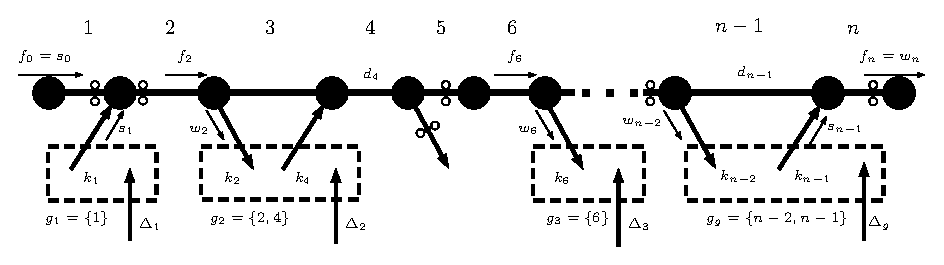
\includegraphics[width=7in]{figures/scheme.eps}
%	\normalsize{
%		\begin{tabular}{llll}
%		\ \ \ \ \ \ \ \ \ \ \ \ \ \ && \ \ \ \ \ \ \ \ \ \ \ \ \ \ & \\ 
%
%			&$L=\llbracket 1,n \rrbracket$ && Mainline link indexes\\
%			&$S\subset{L}$ && Source link indexes (index of preceding 	mainline link)\\
%			&$W\subset{L}$ && Sink (well) link indexes (index of preceding mainline link)\\
%			&$M\subset{L}$ && Monitored mainline links indexes\\
%			&$K=S\cup{W}\backslash M$ && Non-Monitored ramps indexes : the "knob ramps"\\
%			&$G=(g_{i})_{i\in{\llbracket 1,g, \rrbracket}}$ && Knob group indexes\\
%			&$k_{p}=(k_{i_{1}}^{(p)},k_{i_{2}}^{(p)}...,k_{i{\kappa}}^{(p)})$ && Knobs value vector at iteration p\\
%			&$\sigma=(\sigma_{i_{1}},\sigma_{i_{2}}...,\sigma_{i_{\kappa}})$ && $\pm1$ : on- or off-ramp indicator for knobs\\
%			&$(f^{(p)}_{i})_{i\in{L}}$ && Mainline out flows after evaluation p\\
%			&$(s^{(p)}_{i})_{i\in{S}}$ && Source out flows after evaluation p\\
%			&$(w^{(p)}_{i})_{i\in{W}}$ && Sink out flows after evaluation p\\
%			\\
%		\end{tabular}
%	}
%	\rule{7in}{0.3pt}
%	\caption{Freeway model and notation}
%	\label{fig:scheme}
%\end{figure}





\bibliographystyle{IEEEtran}
%\bibliography{bandwidth}

\end{document}